\documentclass{gapd}
\usepackage{amsmath,amsfonts,amsthm} % Math packages for equations
\usepackage{enumitem} % Required for customising lists
\usepackage{caption}
\usepackage{stfloats}
\usepackage{float}

\usepackage{booktabs}%提供命令\toprule、\midrule、\bottomrule

\usepackage{graphicx, subfig}
\usepackage{hyperref}
\hypersetup{hidelinks,
	colorlinks=true,
	allcolors=black,
	pdfstartview=Fit,
	breaklinks=true}

\geometry{a4paper}
\Type{Data Mining in Bioinformatics}
\Title{Prediction of Splicing Sites by BN}

\Author{Jixiong Su}{Undergraduate, Bioinformatics, HUST}


\Abstract{Among the various tools in 
computational genetic research, 
gene prediction remains one of the most 
prominent tasks. Accurate gene prediction is of prime importance 
for the creation and improvement of annotations of sequenced genomes. In this paper, I have developed a model combined WAM and Bayesian Network. Compared with the exsiting model like Weight Array Model and Support Vector Machine, WAM+BN show great performance with excellent predicting accuracy and acceptable balenced time and space expenses.}

%\Pages{35}{37}

\begin{document}
\maketitle

\textbf{Key Words}: Bayesian Network, Machine Learning, Gene Finding, Splice Sites.

\textbf{Availability}: \href{https://github.com/Achuan-2/Splicing-Sites-Predicter}{https://github.com/Achuan-2/Splicing-Sites-Predicter}

\section{INTRODUCTION}\label{introduction}

\lettrine{A}{}  gene is a basic unit of heredity and a sequence of nucleotides in DNA
or RNA that encodes the synthesis of a gene product, either RNA or
protein. Gene prediction or gene finding refers to the process of
identifying the regions of genomic DNA that encode genes. This includes
protein-coding genes as well as RNA genes, but may also include
prediction of other functional elements such as regulatory regions. Gene
finding is one of the first and most important steps in understanding
the genome of a species once it has been sequenced.

In its earliest days, "gene finding" was based on painstaking
experimentation on living cells and organisms. Statistical analysis of
the rates of homologous recombination of several different genes could
determine their order on a certain chromosome, and information from many
such experiments could be combined to create a genetic map specifying
the rough location of known genes relative to each other. Today, with
comprehensive genome sequence and powerful computational resources at
the disposal of the research community, gene finding has been redefined
as a largely computational problem.

Ab Initio gene prediction is an intrinsic method based on \textbf{signal
detection} and \textbf{gene content}. These signs can be broadly
categorized as either signals, specific sequences that indicate the
presence of a gene nearby, or content, statistical properties of the
protein-coding sequence itself. Ab initio gene finding might be more
accurately characterized as gene prediction, since extrinsic evidence is
generally required to conclusively establish that a putative gene is
functional.

In the genomes of prokaryotes, genes have specific and relatively
well-understood promoter sequences (signals), such as the Pribnow box
and transcription factor binding sites, which are easy to systematically
identify. Also, the sequence coding for a protein occurs as one
contiguous open reading frame (ORF), which is typically many hundred or
thousands of base pairs long. Furthermore, protein-coding DNA has
certain periodicities and other statistical properties that are easy to
detect in a sequence of this length. These characteristics make
prokaryotic gene finding relatively straightforward, and well-designed
systems are able to achieve high levels of accuracy.

Ab initio gene finding in eukaryotes, especially complex organisms like
humans, is considerably more challenging for several reasons. First, the
promoter and other regulatory signals in these genomes are more complex
and less well-understood than in prokaryotes, making them more difficult
to reliably recognize. Second, splicing mechanisms employed by
eukaryotic cells mean that a particular protein-coding sequence in the
genome is divided into several parts (exons), separated by non-coding
sequences (introns). A typical protein-coding gene in humans might be
divided into a dozen exons, each less than two hundred base pairs in
length, and some as short as twenty to thirty. It is therefore much more
difficult to detect periodicities and other known content properties of
protein-coding DNA in eukaryotes.

In eukaryotic genes, splice sites mark the boundaries between exons and
introns. Within introns, a donor site (5' end of the intron), a branch
site (near the 3' end of the intron) and an acceptor site (3' end of the
intron) are required for splicing. The splice donor site includes an
almost invariant sequence GU at the 5' end of the intron, within a
larger, less highly conserved region. The splice acceptor site at the 3'
end of the intron terminates the intron with an almost invariant AG
sequence. Upstream (5'-ward) from the AG there is a region high in
pyrimidines (C and U), or polypyrimidine tract. Further upstream from
the polypyrimidine tract is the branchpoint, which includes an adenine
nucleotide involved in lariat formation.

In this paper, I focus on the signal related to pre-mRNA splicing, i.e.
the splice sites that include donor and acceptor sites. However the
occurrence of the dimer in splicing sites is not sufficient for the
splice site. Indeed, it occurs very frequently at non splice site
positions. So we need to construct a model that can analyze the
correlation of the bases upstream and downstream of the splicing sites
to identify splicing sites. I will try to use Bayesian network to
predict splicing sites, compared with other models such as WAM, SVM.

\section{METHODS}\label{methods}

\subsection{Bayesian Network}\label{bayesian-network}

A Bayesian network, Bayes network, belief network, Bayes(ian) model or
probabilistic directed acyclic graphical model is a probabilistic
graphical model (a type of statistical model) that represents a set of
random variables and their conditional dependencies via a directed
acyclic graph (DAG). Bayesian networks are mostly used when we want to
represent causal relationship between the random variables. Bayesian
Networks are parameterized using Conditional Probability Distributions
(CPD). Each node in the network is parameterized using $ P(node | Pa(node)) $ where $Pa(node) $ represents the parents of node in the network.

From the Bayesian rule, the global joint distribution function 
$P\left(x_{1}, x_{2}, \ldots, x_{n}\right)$ of variables $X_{1}, X_{2}, \ldots, X_{n}$ 
can be represented as a product of local conditional distribution functions. That is,
\begin{equation*}
  \begin{aligned}
  P\left(x_{1}, x_{2}, \ldots, x_{n}\right) =  P\left(x_{1}\right) P\left(x_{2} \mid x_{1}\right) \cdots 
  P\left(x_{n} \mid x_{1}, \ldots, x_{n-1}\right) 
  \end{aligned}  
\end{equation*}

A Bayesian network for a collection $\{X_{1}, X_{2}, \ldots, X_{n}\}$ of random variables
represents the joint probability distribution of these variables.
The joint probability distribution, which is associated with a set of assertions of conditional independence among the variables, can be written as:
$$
P\left(x_{1}, x_{2}, \ldots, x_{n}\right)=\prod_{i=1}^{n} P\left(x_{i} \mid E_{x_{i}}\right)
$$
where $E_{x_{i}}$ is a subset of variables $x_{1}, \ldots, x_{i-1}$
on which $x_{i}$ is dependent.
Hence, a Bayesian network can be described as a directed acyclic
graph consisting of a set of $n$ nodes and a set of
directed edges between nodes. 
Each node in the graph corresponds to a variable $x_{i}$ and 
each directed edge is constructed from a variable 
in $E_{x_{i}}$ to the variable $x_{i} .$ 
If each variable has a finite set of values, to each variable
$x_{i}$ with parents in $E_{x_{i}}$, 
there is an attached table of conditional probabilities 
$P\left(x_{i} \mid E_{x_{i}}\right) .$

\subsection{Program Design}\label{program-design}

\paragraph{Step 1: Feature Extraction and
Encoding}\label{feature-extraction-and-encoding}

Extract sequences from training set and test set and then extract
windows with fixed length that contains a donor splice site, excluding
the windows that contained base positions not labeled with A, T, C, G but
with other symbols. Finally encode sequences with the rule that
\textbf{A is encoded for 0, G for 1, C for 2, T for 3}.

\paragraph{Step 2: Define the network
structure}\label{define-the-network-structure}

I use \textbf{pgmpy} for model architecture. pgmpy is a python library
for working with Probabilistic Graphical Models. In pgmpy we define the
network structure and the CPDs separately and then associate them with
the structure. And I use the \textbf{HillClimbSearch} function to
estimate the structure, which performs local hill climb search to
estimates the DAG structure that has optimal score, according to the
scoring method supplied. Starts at model start\_dag and proceeds by
step-by-step network modifications until a local maximum is reached.

\paragraph{Step 3: Model architecture and Parameter
Learning}\label{model-architecture-and-parameter-learning}

According to a DAG and features from training set ( label positive samples
as 1 and negative as 0 ), build a Bayesian model and estimate the
(conditional) probability distributions of the individual variables.

For model architecture, the network have \textbf{two kinds of nodes}:
the feature nodes \(N_i\) and label node \(N_{Label}\).In the Bayesian
network, each feature node has state \({Base} \in\) \(\{a, c, g, t\}\)
and label node has state \({Label} \in\{0,1\}\). To enable Bayesian
network to learn conditional probability for all nodes, both donor
sites and pseudo sites are fitted in a Bayesian network.

For parameter learning, I use \textbf{Bayesian Parameter Estimation}.The
Bayesian Parameter Estimator starts with already existing prior CPDs,
that express our beliefs about the variables \emph{before} the data was
observed. Those "priors" are then updated, using the state counts from
the observed data. A sensible choice of prior is \emph{BDeu} (Bayesian
Dirichlet equivalent uniform prior). For BDeu we need to specify an
equivalent sample size N and then the pseudo-counts are the equivalent
of having observed N uniform samples of each variable (and each parent
configuration).

\paragraph{Step 4: Prediction and score}\label{prediction-and-score}

Input all samples from test set with missing label, predict
probabilities of label 1 and label 0. The score, \(Score(S)\), of a
tested potential splice site S under the two labels is the log-odds
ratio defined as follows:

\[Score(S)=\log \left[\frac{P\left(S \mid Label_{\mathrm{1}}\right)}{P\left(S \mid Label_{\mathrm{0}}\right)}\right]\]
With an empirically determined threshold score T , the tested potential
splice site S will be claimed real if the log-odds score is no less than
T ; otherwise, it will be claimed pseudo signal.

\paragraph{Step 5: Evaluation}\label{evaluation}

Compare the performance of Bayesian Network with other models such as
WAM and SVM by ROC curve and PR curve.

Receiver operating characteristic Curve (ROC Curve for short) is a curve
reflecting the relationship between sensitivity and specificity. The
closer the ROC curve is to the upper left corner, the higher the
accuracy of the test. The point closest to the top left corner of the
ROC curve is the best threshold. AUC is the
area under the ROC curve. The meaning of AUC value is to randomly
take a pair of positive and negative samples, and the probability that
the score of positive samples is greater than that of negative samples.
AUC is robust to the unbalanced distribution of positive and negative
samples, and it is a very common measure of classifier.

Precision-Recall Curve is a useful measure of success of prediction when the
classes are very imbalanced (PR curve for short). In information
retrieval, precision is a measure of result relevancy, while recall is a
measure of how many truly relevant results are returned. When the
distribution of positive and negative samples is unbalanced, the ROC
curve remains unchanged, while the PR curve changes greatly. Compared
with the ROC curve, the PR curve can reflect the ability of the model to
identify positive samples. AUROC is always going to be 0.5 --- a random
classifier, or a coin toss, will get you an AUROC of 0.5. But with
AUPRC, the baseline is equal to the fraction of positives.

Other measures of predictive accuracy are as follows:

\begin{gather*}%不会产生编号
  Sn/Recall = \frac{TP}{TP+FN} \\
  Precision = \frac{TP}{TP+FP} \\
  F1\text{-}score =2* \frac{Precision*Recall}{Precision+Recall}
\end{gather*}



\begin{figure}
  \centering
  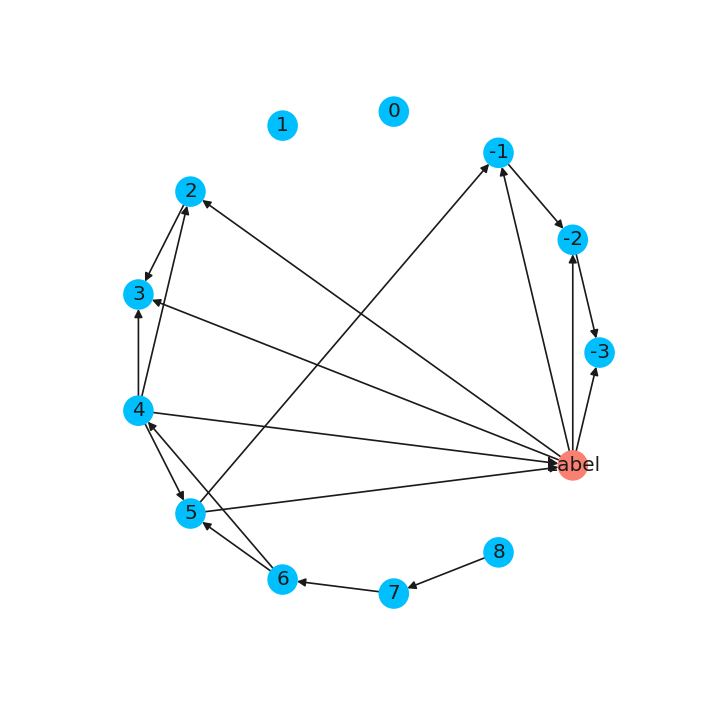
\includegraphics[width=\columnwidth]{assets/network-20210609212835-4n4fayy.png}
  \caption{The Bayesian Network Structure}
  \label{fig:network}
\end{figure}  



\section{RESULTS}\label{results}

\subsection{Splice Site Datasets}\label{splice-site-datasets}

The Kulp-Reese dataset is used as a training set, which consists of
462 non-redundant multi-exon genes, is a benchmark data set and has been
widely used to train many powerful gene prediction algorithms.

The Test set is Burset \& Guigo set. The dataset assembled by Burset
and Guigo(1996) consists of 570 vertebrate genomic sequences containing
exaxctly multi-exon gene. There are 2079 exons and introns in the whole
dataset, with more than 140000 pseudo exons and introns in the dataset.
( the testing dataset can be found at
\url{https://genome.crg.cat/datasets/genomics96/})



\subsection{Bayesian Network Results}\label{bayesian-network-results}


Choose a window that contains 3 consecutive bases upstream from the
exon/intron boundary and 9 consecutive bases downstream to the
exon/intron boundary. Build a model by pgmpy. The network obtained is
shown in Figure\ref{fig:network}.



Using the Bayesian network to train model, ROC and PR curves and
confusion matrixes are shown in  Figure\ref{fig:BNmatrix} and Figure\ref{fig:WBROC}. It can be seen from ROC
and PR curves that the performance of this model is ordinary. Although
we consider the correlation of all bases, the performance of the model
is not significantly improved compared with WAM.


\begin{figure}[hb]
  \centering
  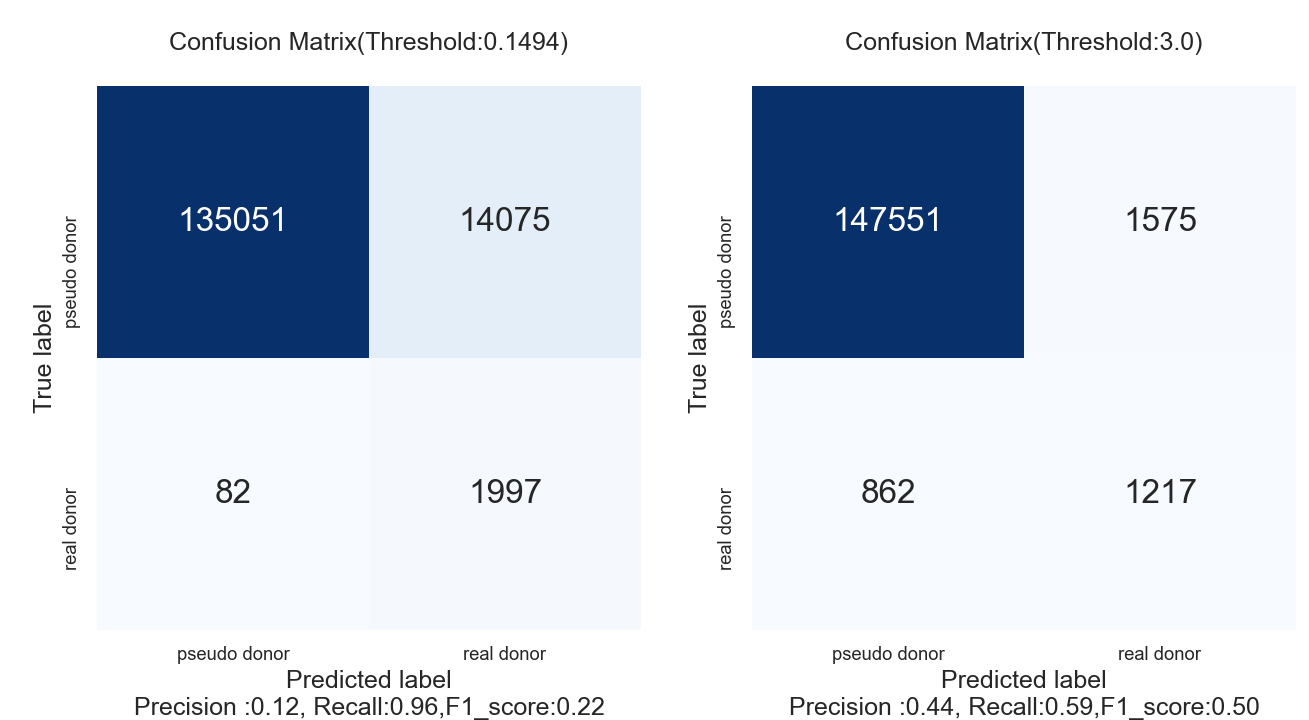
\includegraphics[width=\columnwidth]{assets/image-20210624154725944.png}
  \caption{Confusion Matrix for Bayesian Network: The left is under the threshold is
  the best parameter of ROC curve. The right is under the threshold when
  F1-score is highest.}
  \label{fig:BNmatrix}
\end{figure}

\begin{table*}
  \centering
  \caption{Prediction under different thresholds in Bayesian network}
  \begin{tabular}{cccccccccc}
  \hline
\toprule%第一道横线
      Threshold & TP & FP & TN & FN & Recall & Precision & F1-Score & Sn & Acc \\ 
\midrule%第二道横线
      -10 & 2079 & 142390 & 6736 & 0 & 1.000 & 0.014 & 0.028 & 0.045 & 0.058 \\ 
      -9 & 2079 & 134157 & 14969 & 0 & 1.000 & 0.015 & 0.030 & 0.100 & 0.113 \\ 
      -8 & 2078 & 124224 & 24902 & 1 & 1.000 & 0.016 & 0.032 & 0.167 & 0.178 \\ 
      -7 & 2078 & 114803 & 34323 & 1 & 1.000 & 0.018 & 0.035 & 0.230 & 0.241 \\ 
      -6 & 2078 & 104199 & 44927 & 1 & 1.000 & 0.020 & 0.038 & 0.301 & 0.311 \\ 
      -5 & 2078 & 90422 & 58704 & 1 & 1.000 & 0.022 & 0.044 & 0.394 & 0.402 \\ 
      -4 & 2075 & 74324 & 74802 & 4 & 0.998 & 0.027 & 0.053 & 0.502 & 0.508 \\ 
      -3 & 2070 & 56339 & 92787 & 9 & 0.996 & 0.035 & 0.068 & 0.622 & 0.627 \\ 
      -2 & 2065 & 41259 & 107867 & 14 & 0.993 & 0.048 & 0.091 & 0.723 & 0.727 \\ 
      -1 & 2048 & 25702 & 123424 & 31 & 0.985 & 0.074 & 0.137 & 0.828 & 0.830 \\ 
      0 & 2010 & 15492 & 133634 & 69 & 0.967 & 0.115 & 0.205 & 0.896 & 0.897 \\ 
      1 & 1882 & 7689 & 141437 & 197 & 0.905 & 0.197 & 0.323 & 0.948 & 0.948 \\ 
      1.5 & 1810 & 5604 & 143522 & 269 & 0.871 & 0.244 & 0.381 & 0.962 & 0.961 \\ 
      2 & 1672 & 3887 & 145239 & 407 & 0.804 & 0.301 & 0.438 & 0.974 & 0.972 \\ 
      3 & 1217 & 1575 & 147551 & 862 & 0.585 & 0.436 & 0.500 & 0.989 & 0.984 \\ 
      4 & 684 & 571 & 148555 & 1395 & 0.329 & 0.545 & 0.410 & 0.996 & 0.987 \\ 
      4.5 & 440 & 266 & 148860 & 1639 & 0.212 & 0.623 & 0.316 & 0.998 & 0.987 \\ 
      5 & 267 & 122 & 149004 & 1812 & 0.128 & 0.686 & 0.216 & 0.999 & 0.987 \\ 
      5.1 & 195 & 82 & 149044 & 1884 & 0.094 & 0.704 & 0.166 & 0.999 & 0.987 \\ 
      5.5 & 65 & 42 & 149084 & 2014 & 0.031 & 0.607 & 0.059 & 1.000 & 0.986 \\ 
      5.8 & 27 & 22 & 149104 & 2052 & 0.013 & 0.551 & 0.025 & 1.000 & 0.986 \\ 
      5.9 & 11 & 14 & 149112 & 2068 & 0.005 & 0.440 & 0.010 & 1.000 & 0.986 \\ 
      6.2 & 0 & 0 & 149126 & 2079 & 0.000 &  &  & 1.000 & 0.986 \\ 
\bottomrule%第三道横线
  \end{tabular}
\end{table*}

\subsection{WAM+Bayesian Network}\label{wambayesian-network}

In view of the unsatisfactory effect of Bayesian network, I try to use
WAM to filter out the samples with large difference between negative
samples and positive samples, and then use Bayesian network to train and
predict the input positive and negative samples, i.e., I hope
Bayesian network can separate the samples with similar scores in
positive and negative samples in WAM.


During training, the positive and negative samples in the training set
whose score is less than the threshold are filtered out, and then the
Bayesian network is used to train with the filtered samples. In the
process of prediction, WAM is used to score the samples whose score is
less than the threshold value, and the samples whose score is higher
than the threshold value are predicted as negative samples. Finally
Bayesian network is used to predict the samples whose score is higher
than the threshold value.

\begin{figure}[h]
  \centering
  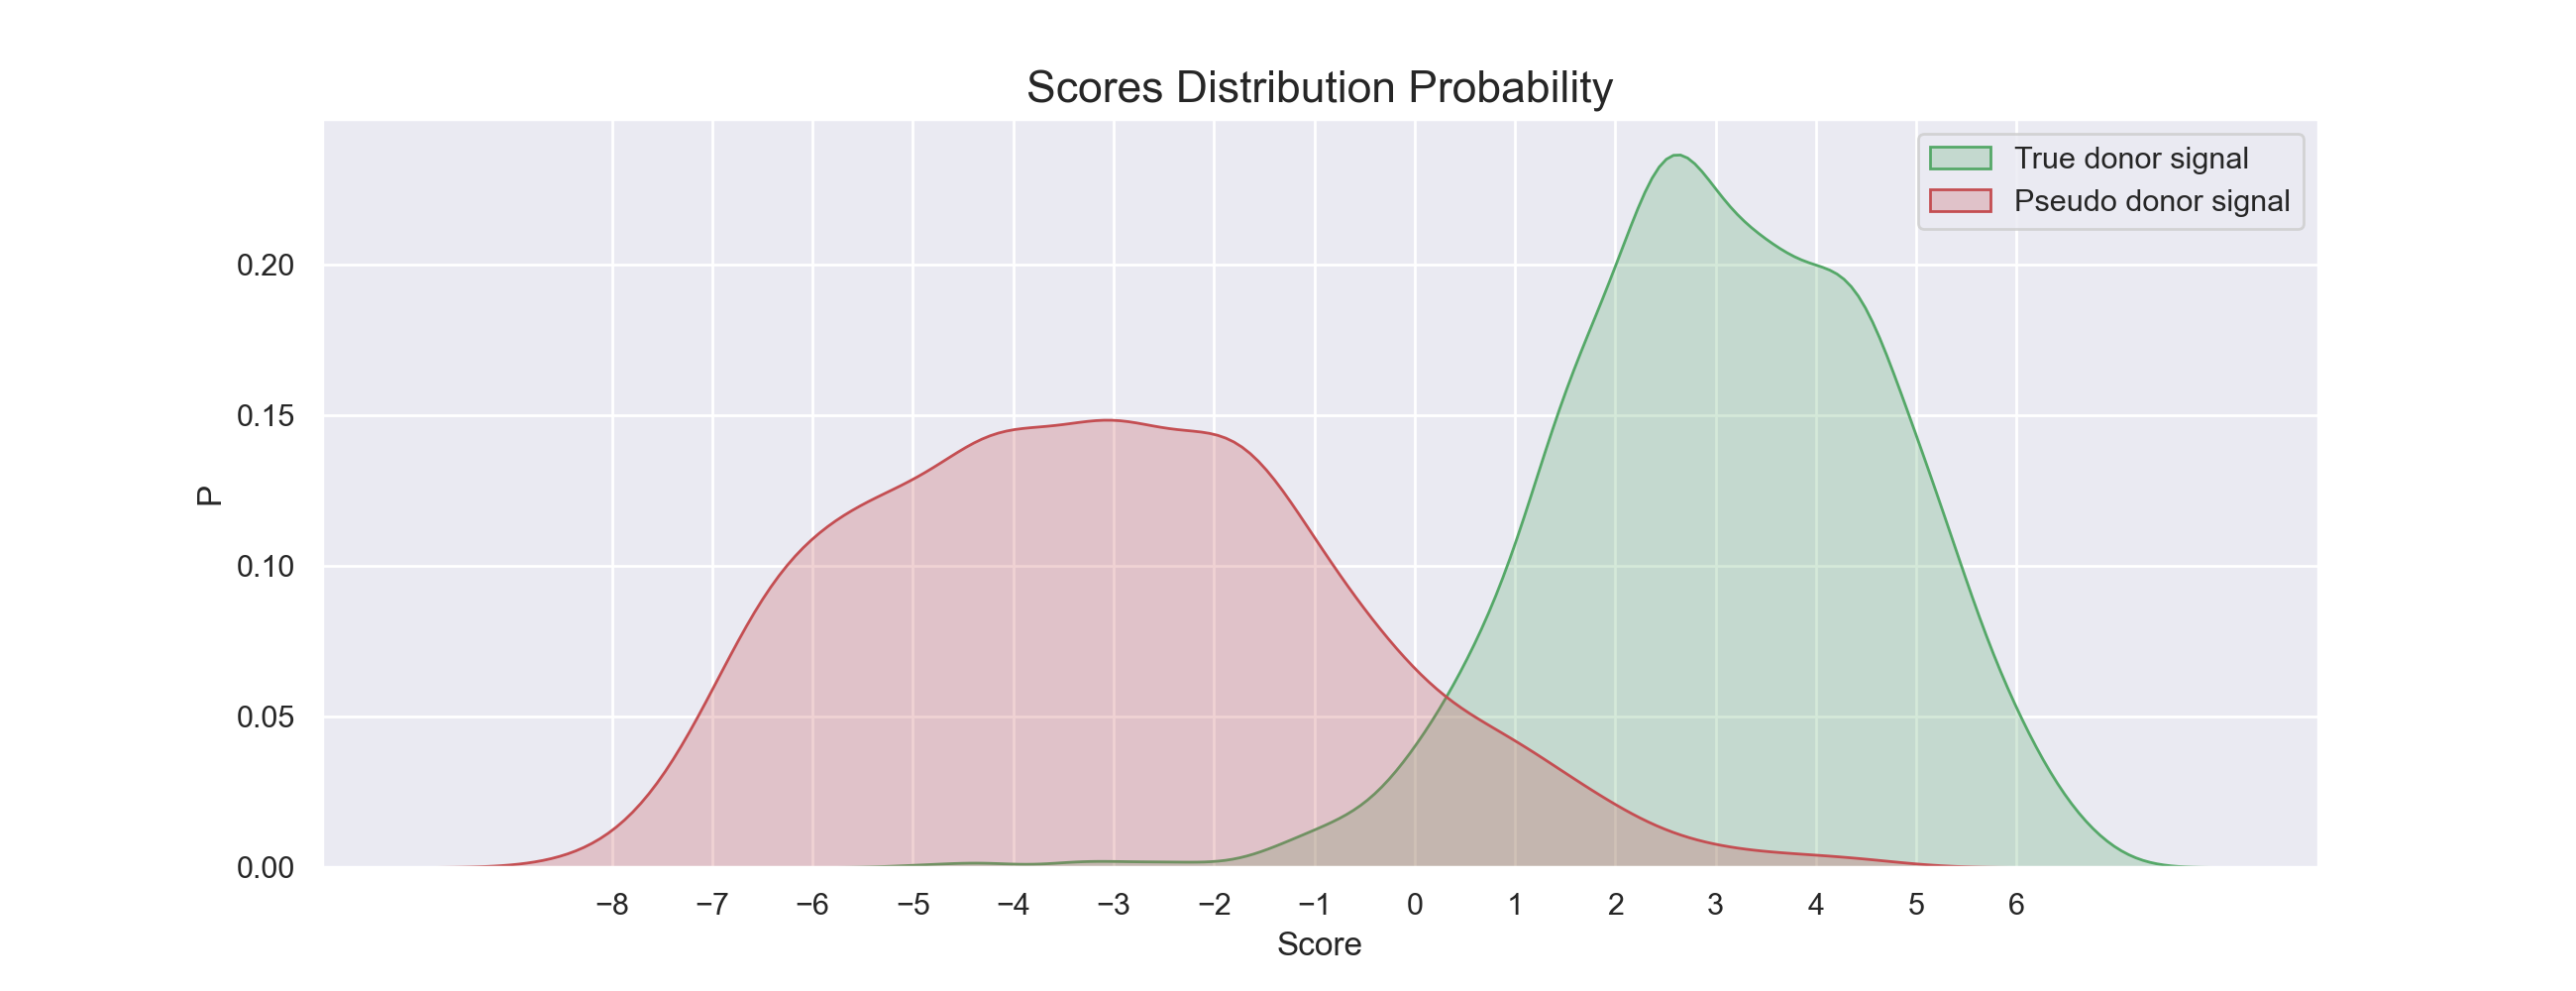
\includegraphics[width=\columnwidth]{assets/Distribution_Probability.png}
  \caption{The scoring of positive and negative samples input 
  from the training set by WAM in the first layer.}
  \label{fig:WBDistribution}
\end{figure}

According to Figure \ref*{fig:WBDistribution}, I set the threshold value of the first layer WAM to - 3, and the result
is excellent. As can be seen from Figure \ref{fig:WBROC} and Figure \ref{fig:WBPRC}, the AUROC of WAM+BN
is 0.988, close to the SVM Poly Kernel preformance. Compared with WAM
and BN, the PR curve has been greatly improved, although it is worse
than SVM Poly Kernel.

\begin{table*}[hbp]
  \centering
  \caption{Prediction under different thresholds in WAM+Bayesian}
  \begin{tabular}{cccccccccc}
  \toprule%第一道横线
      Threshold & TP & FP & TN & FN & Recall & Precision & F1-Score & Sn & Acc \\ 
      \midrule%第二道横线
      -7 & 2077 & 34920 & 114206 & 2 & 0.999 & 0.056 & 0.106 & 0.766 & 0.769 \\ 
      -6 & 2077 & 34174 & 114952 & 2 & 0.999 & 0.057 & 0.108 & 0.771 & 0.774 \\ 
      -5 & 2077 & 32867 & 116259 & 2 & 0.999 & 0.059 & 0.112 & 0.780 & 0.783 \\ 
      -4 & 2076 & 30756 & 118370 & 3 & 0.999 & 0.063 & 0.119 & 0.794 & 0.797 \\ 
      -3 & 2070 & 26914 & 122212 & 9 & 0.996 & 0.071 & 0.133 & 0.820 & 0.822 \\ 
      -2 & 2063 & 20733 & 128393 & 16 & 0.992 & 0.090 & 0.166 & 0.861 & 0.863 \\ 
      -1 & 2052 & 14321 & 134805 & 27 & 0.987 & 0.125 & 0.222 & 0.904 & 0.905 \\ 
      0 & 1993 & 8345 & 140781 & 86 & 0.959 & 0.193 & 0.321 & 0.944 & 0.944 \\ 
      1 & 1880 & 3874 & 145252 & 199 & 0.904 & 0.327 & 0.480 & 0.974 & 0.973 \\ 
      1.5 & 1751 & 2666 & 146460 & 328 & 0.842 & 0.396 & 0.539 & 0.982 & 0.980 \\ 
      2 & 1590 & 1761 & 147365 & 489 & 0.765 & 0.474 & 0.586 & 0.988 & 0.985 \\ 
      3 & 1049 & 685 & 148441 & 1030 & 0.505 & 0.605 & 0.550 & 0.995 & 0.989 \\ 
      4 & 467 & 200 & 148926 & 1612 & 0.225 & 0.700 & 0.340 & 0.999 & 0.988 \\ 
      4.5 & 224 & 94 & 149032 & 1855 & 0.108 & 0.704 & 0.187 & 0.999 & 0.987 \\ 
      5 & 88 & 40 & 149086 & 1991 & 0.042 & 0.688 & 0.080 & 1.000 & 0.987 \\ 
      5.5 & 8 & 6 & 149120 & 2071 & 0.004 & 0.571 & 0.008 & 1.000 & 0.986 \\ 
      5.6 & 3 & 2 & 149124 & 2076 & 0.001 & 0.600 & 0.003 & 1.000 & 0.986 \\ 
      5.7 & 0 & 0 & 149126 & 2079 & 0.000 &  &  & 1.000 & 0.986 \\ 
      \bottomrule%第三道横线
  \end{tabular}
\end{table*}


\begin{figure}[hb]
  \centering
  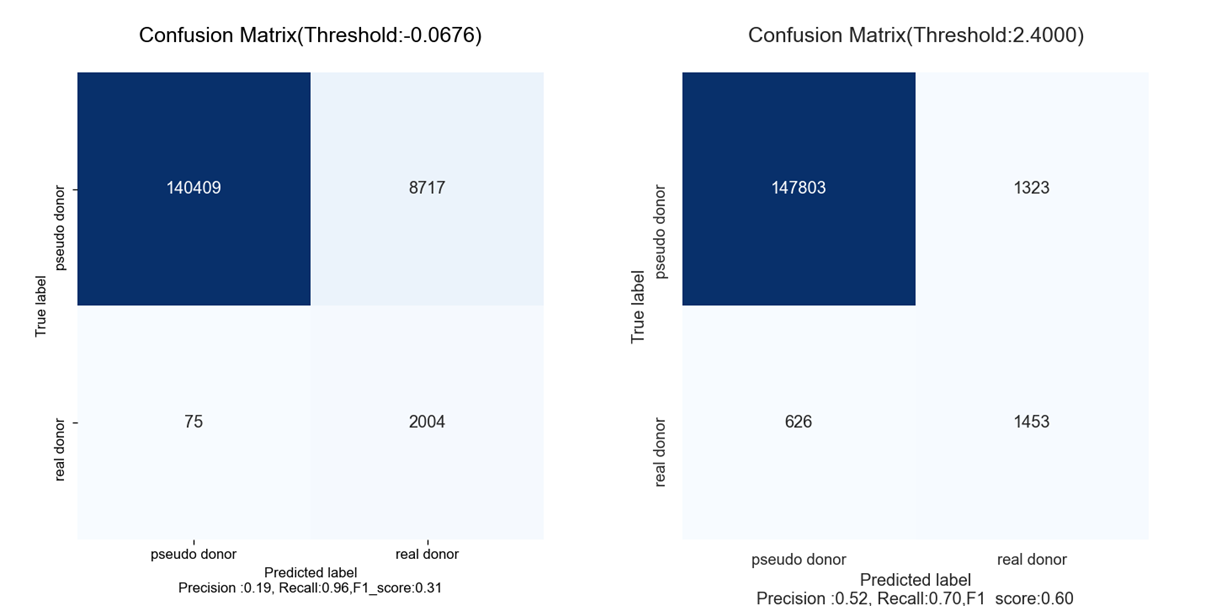
\includegraphics[width=\columnwidth]{assets/image-20210624154819817.png}
  \caption{Confusion Matrix for WAM+Bayesian: The left is under the
  threshold is the best parameter of ROC curve. The right is under the
  threshold when F1-score is highest.}
  \label{fig:WBmatrix}
\end{figure}

\begin{figure*}[htbp]
  \centering
  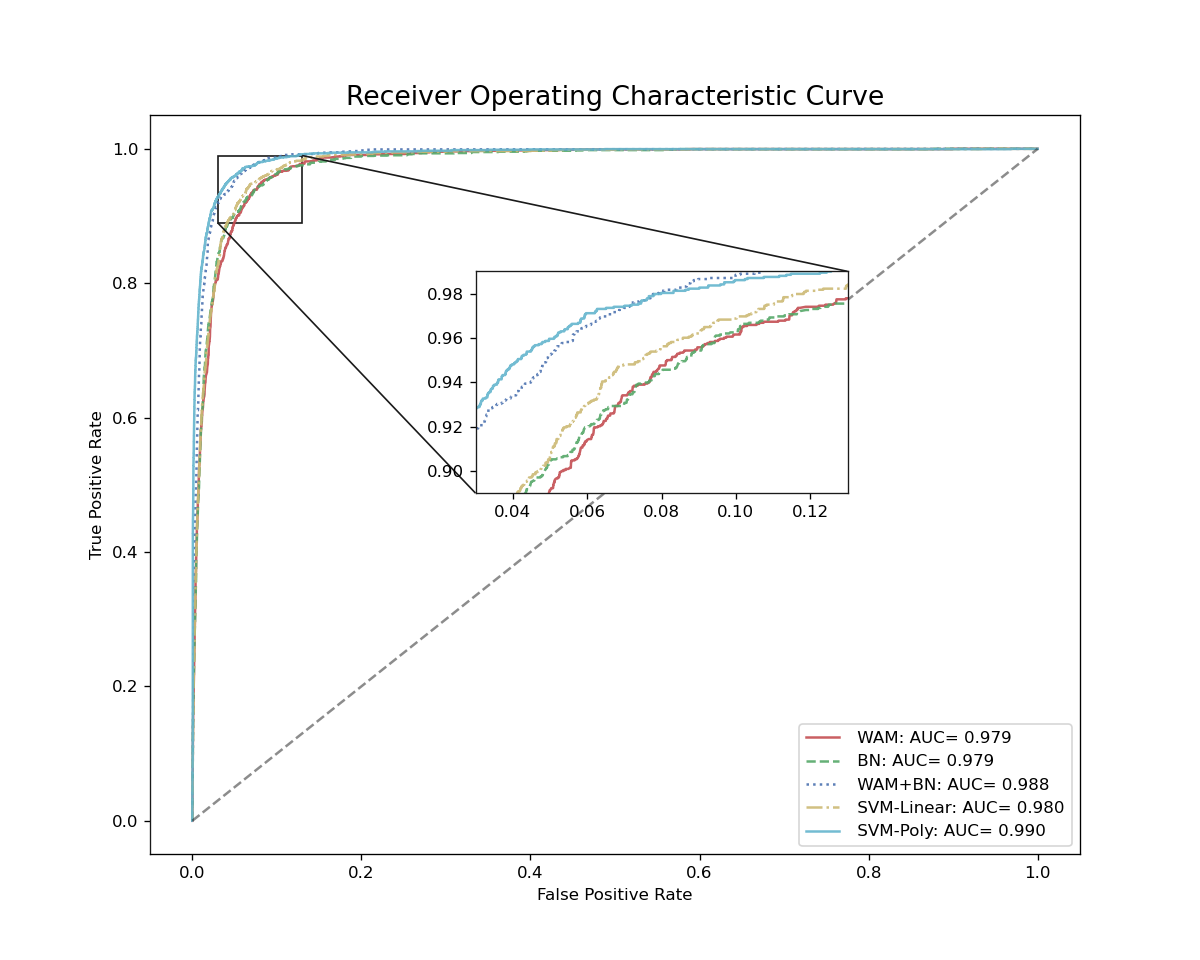
\includegraphics[width=0.8\linewidth]{assets/ROC_plot.png}
  \caption{Receiver Operating Charateristic Curve  for Bayesian, WAM+Bayesian Network and other models}
  \label{fig:WBROC}
\end{figure*}
\begin{figure*}[htbp]
  \centering
  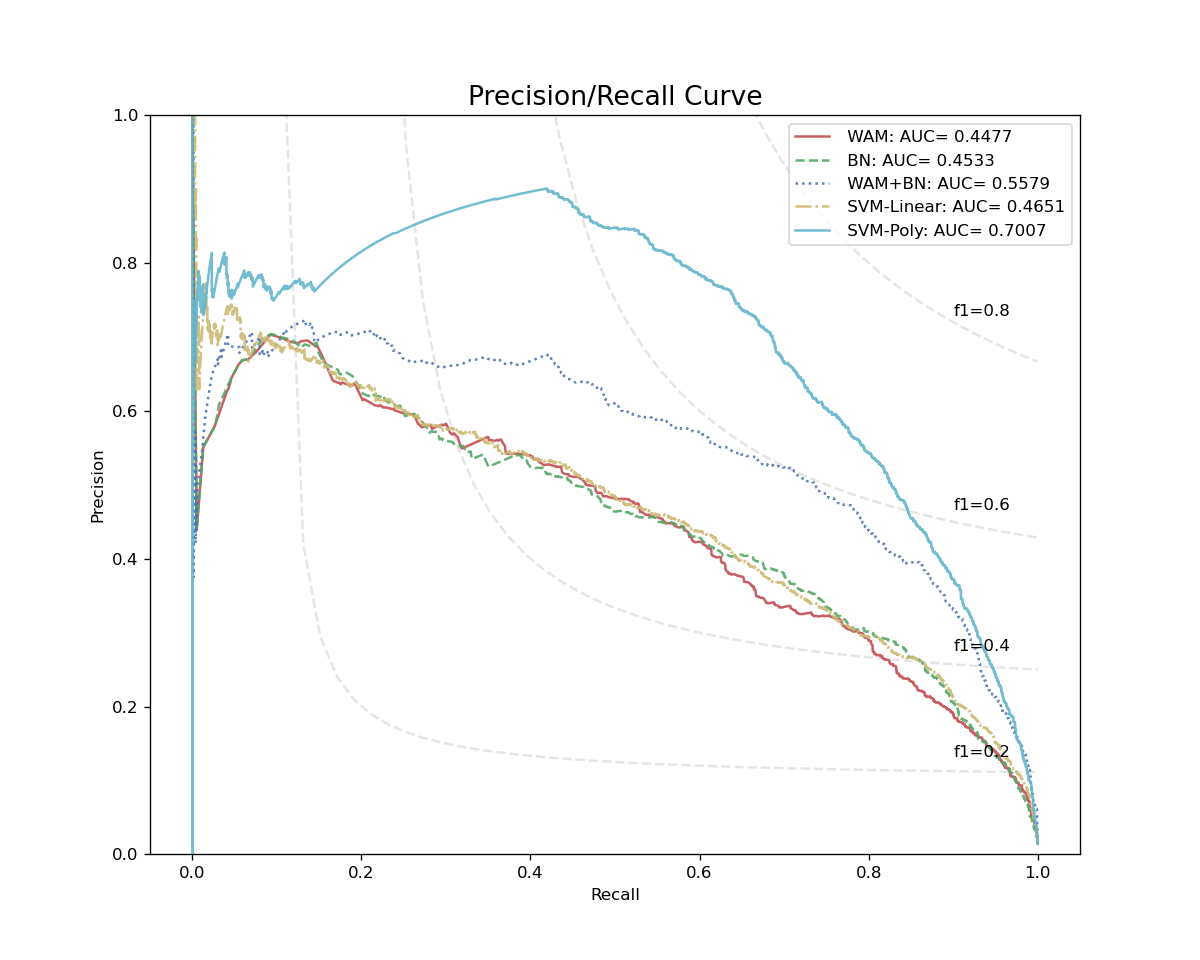
\includegraphics[width=0.8\linewidth]{assets/PR_plot.png}
  \caption{R Precison/Recall
  Curve for Bayesian, WAM+Bayesian Network and other models}
  \label{fig:WBPRC}
\end{figure*}



\section{DISCUSSION \& CONCLUSION}\label{discussion--conclusion}

In this study, I firstly use Bayesian Network to build a model to
predict donor sites, in view of the effect compared with WAM, almost no
improvement. So I try WAM + BN to build a two-layer model, which can be
compared with SVM. At first, the effect of only using Bayesian network
is poor, which may be due to the unbalanced number of positive and
negative samples. Bayesian Network constructs conditional probability
matrix according to the situation of samples and network structure. When
the number of samples is too large, the network will be too complex and
eventually the discrimination between positive and negative samples is
not high. After one-layer filtering by WAM, the number of input Bayesian
network samples is reduced, which reduces the time and space cost of
training. The samples that the first layer of WAM can not distinguish
the samples well, using more complex Bayesian network to train and
predict, making the Bayesian network only for the samples that are
difficult to distinguish. It has been proved that this method has
greatly improved the prediction accuracy of the model.



\section{ACKNOWLEDGEMENTS}\label{acknowledgements}

Thank Professor Yanhong Zhou for his patient guidance. The computing
work in this paper is mostly supported by the public computing service
platform provided by Network and Computing Center of HUST.

\section{REFERENCES}\label{references}

\begin{enumerate}
  \item
    Te-Ming Chen, Chung-Chin Lu, Wen-Hsiung Li, Prediction of splice sites
    with dependency graphs and their expanded bayesian networks,
    \emph{Bioinformatics}, Volume 21, Issue 4, 15 February 2005, Pages
    471--482, 
  \item
    Cai D, Delcher A, Kao B, Kasif S. Modeling splice sites with Bayes
    networks. Bioinformatics. 2000 Feb;16(2):152-8. doi:
    10.1093/bioinformatics/16.2.152. PMID: 10842737.
\end{enumerate}
\end{document}